\documentclass[a4paper,14pt]{extarticle}

\usepackage[left=30mm, right=10mm, top=20mm, bottom=20mm]{geometry}

\usepackage{amssymb}
\usepackage{amsmath}
\usepackage{tikz}
\usepackage{pgfplots}

\usepackage{graphicx}
\usepackage{setspace}

\usepackage{minted}
\usepackage{xcolor}

\usepackage{siunitx}
\usepackage{booktabs}
\usepackage{multirow}

\usepackage[T2A]{fontenc}
\usepackage[utf8]{inputenc}
\usepackage[russian]{babel}
\usepackage{tempora}
\usepackage{type1cm}
\usepackage{indentfirst}

\usepackage{caption}
\usepackage{subcaption}
\usepackage[hidelinks]{hyperref}
\usepackage[russian]{cleveref}
\usepackage{bookmark}

\pgfplotsset{compat=1.18}

\onehalfspacing

\renewcommand{\theFancyVerbLine}{%
	\sffamily\small\color{black}\arabic{FancyVerbLine}%
}

\definecolor{codebg}{rgb}{0.12,0.12,0.14}
\definecolor{codeframe}{rgb}{0.40,0.40,0.45}
\definecolor{keywordcolor}{rgb}{0.45,0.65,1.0}
\definecolor{stringcolor}{rgb}{1.0,0.55,0.45}
\definecolor{commentcolor}{rgb}{0.55,0.75,0.60}
\definecolor{textcolor}{rgb}{0.90,0.90,0.90}

\setminted{
    bgcolor=codebg,
	fillcolor=codebg,
	framesep=1em,
	frame=single,
    rulecolor=\color{codeframe},
    fontsize=\normalsize,
    baselinestretch=1.1,
    linenos,
    numbersep=6pt,
    tabsize=4,
    breaklines,
    breakbytoken,
	breaksymbolleft={},
    autogobble,
    showspaces=false,
    showtabs=false,
}

\usemintedstyle{lightbulb}
\setmintedinline{
    bgcolor=codebg
}

\makeatletter
\setlength{\@fptop}{0pt}
\setlength{\@fpsep}{8pt}
\setlength{\@fpbot}{0pt plus 1fil}
\makeatother

\newcommand{\circledequals}{\mathbin{\tikz \node[draw,circle,inner sep=1pt] {$=$};}}

\DeclareMathOperator{\Bernoulli}{Bernoulli}

\begin{document}
    \begin{titlepage}
		\centering
		
		
\includegraphics{images/FEFU-logo.jpg}\\
		МИНИСТЕРСТВО ОБРАЗОВАНИЯ И НАУКИ РОССИЙСКОЙ ФЕДЕРАЦИИ\\
		Федеральное государственное автономное образовательное учреждение высшего образования\\
		\textbf{«Дальневосточный федеральный университет»}

		\rule{\linewidth}{0.8mm}\\[0.3cm]
		
		\textbf{ИНСТИТУТ МАТЕМАТИКИ И КОМПЬЮТЕРНЫХ ТЕХНОЛОГИЙ}\\
		\textbf{Кафедра математического и компьютерного моделирования}\\
		\vspace*{0.9cm}
		
		Кулахсзян Сергей Грайрович\\
        \vspace*{0.3cm}

		ВАРИАНТ № 18 \\
		\vspace*{0.3cm}

		\textbf{ИНДИВИДУАЛЬНАЯ ДОМАШНЯЯ РАБОТА}\\
		\vspace*{0.3cm}

		Направление подготовки 02.03.01сцт Сквозные цифровые технологии,\\ 
        бакалавриатская программа «Математика и компьютерные науки»\\ 
        Очной формы обучения\\
		\vspace{1.5cm}

		
		\vfill
		\centering
		г. Владивосток\\
		2026
	\end{titlepage}

    \tableofcontents
	\newpage

	\section{задание}

	\subsection{Входные данные}

	\begin{equation} \label{X_18_1}
		\begin{array}{cccccccccc}
			X_{18}: \\
			12.67 & 15.16 & 2.69 & 16.37 & 6.24 & 10.17 & 15.18 & 5.77 & 5.66 & 8.02 \\
			9.98 & 7.15 & 3.40 & 6.57 & 7.98 & 4.81 & 6.81 & 14.04 & 5.36 & 14.96 \\
			9.46 & 13.27 & 3.64 & 5.96 & 2.95 & 2.78 &7.99 & 9.53 & 5.96 & 9.46 \\
			9.55 & 5.46 & 11.34 & 10.43 & 9.85 & 9.20 & 7.88 & 6.46 & 12.86 & 11.20 \\
			6.48 & 7.20 & 4.29 & 8.34 & 5.57 & 11.80 & 10.32 & 3.70 & 8.77 & 9.33 \\
			4.49 & 5.05 & 6.32 & 14.19 & 11.08 & 7.94 & 11.12 & 1.88 & 9.11 & 11.39 \\
			5.70 & 5.90 & 4.43 & 11.75 & 8.37 & 6.15 & 7.04 & 10.28 & 8.71 & 4.02 \\
			11.92 & 16.16 & 5.45 & 14.84 & 9.55 & 13.25 & 8.08 & 3.15 & 6.27 & 7.21\\
			14.24 & 7.64 & 7.97 & 4.75 & 15.31 & 13.85 & 4.86 & 8.47 & 6.44 & 4.75 \\
			9.25 & 7.83 & 8.03 & 7.60 & 6.13 & 7.19 & 13.23 & 4.86 & 3.49 & 4.68
		\end{array}
	\end{equation}

	\subsection{Интервальный ряд}

	Для составления интервального вариационного ряда для начала необходимо вычислить число интервалов, это делается по формуле Стерджеса: \\
	\[
		k = 1 + 3.332 \cdot \lg(N),
	\]
	где $N = 100$ -- объём выборки. Для нашей работы $k = 7$.

	Тогда интервальный для совокупности $X_{18}$ будет иметь вид:
	\begin{table}[!ht]
		\caption{Интервальный вариационный ряд совокупности $X_{18}$ (\ref{X_18_1})}
		\label{interval_row}
		\begin{tabular}{|l|l|l|}
		\hline
			\textbf{Интервал} & \textbf{Частота, $m_i$} & \textbf{Относительная частота, $n_i$} \\ \hline
			[1.88; 3.95) & 9 & 0.09 \\ \hline
			[3.95; 6.02) & 21 & 0.21 \\ \hline
			[6.02; 8.09) & 26 & 0.26 \\ \hline
			[8.09; 10.16) & 16 & 0.16 \\ \hline
			[10.16; 12.23) & 12 & 0.12 \\ \hline
			[12.23; 14.3) & 9 & 0.09 \\ \hline
			[14.3; 16.37] & 7 & 0.07 \\ \hline
		\end{tabular}
	\end{table}

	Код для построения интервального ряда:
	\begin{minted}{python}
		N = len(X_N)
		k = int(1 + 3.322 * np.log10(N))
		counts, bins = np.histogram(X_N, bins=k)

		intervals = [f"[{bins[i]}; {bins[i+1]})" for i in range(k)]
		intervals[-1] = intervals[-1][:-1] + "]"
		interval_series = pd.DataFrame({
			r'Интервал': intervals,
			r'Частота $m_i$': counts,
			r'Относительная частота $n_i$': counts / N,
		})
		print("Интервальный вариационный ряд:")
		print(interval_series.to_string(index=False))
	\end{minted}

	\subsection{Гистограмма частот}

	Исходя из данных полученных в интервальном ряде (\ref{interval_row}), можно построить гистограмму частот:
	\begin{figure}[!ht]
		\centering
		\caption{Гистограмма частот совокупности $X_{18}$ (\ref{X_18_1})}
		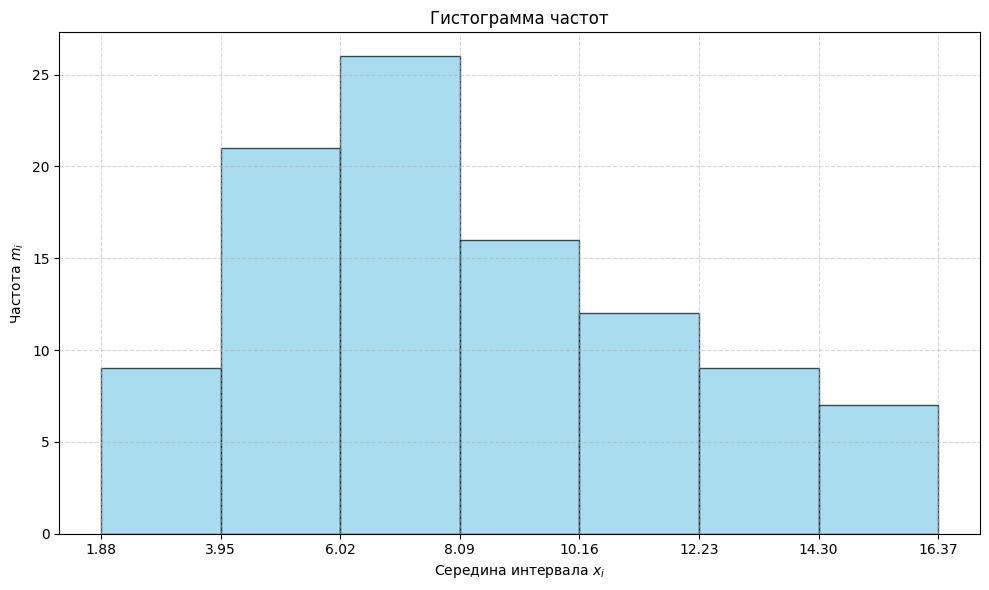
\includegraphics[width=\textwidth]{images/1_histogram.png}
	\end{figure}

	Код:
	\begin{minted}{python}
		plt.figure(figsize=(10, 6))
		plt.hist(X_N, bins=bins, edgecolor='black', alpha=0.7, color='skyblue', density=False)
		plt.title('Гистограмма частот')
		plt.xlabel(r'Середина интервала $x_i$')
		plt.ylabel(r'Частота $m_i$')
		plt.xticks(np.round(bins, 2))
		plt.grid(True, linestyle='--', alpha=0.5)
		plt.tight_layout()
	\end{minted}

	\subsection{Полигон частот}

	Исходя из данных полученных в интервальном ряде (\ref{interval_row}), можно построить полигон частот:
	\begin{figure}[!ht]
		\centering
		\caption{Полигон частот совокупности $X_{18}$ (\ref{X_18_1})}
		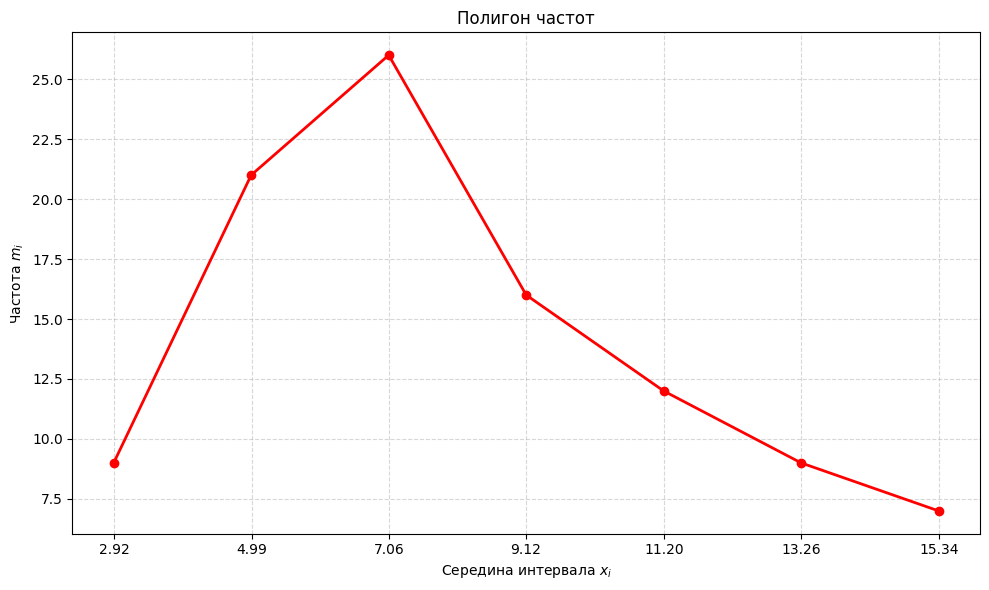
\includegraphics[width=\textwidth]{images/1_polygon.png}
	\end{figure}

	Код:
	\begin{minted}{python}
		bin_centers = (bins[:-1] + bins[1:]) / 2
		plt.figure(figsize=(10, 6))
		plt.plot(bin_centers, counts, marker='o', linestyle='-', color='red', linewidth=2)
		plt.title('Полигон частот')
		plt.xlabel(r'Середина интервала $x_i$')
		plt.ylabel(r'Частота $m_i$')
		plt.xticks(np.round(bin_centers, 2))
		plt.grid(True, linestyle='--', alpha=0.5)
		plt.tight_layout()
	\end{minted}

	\subsection{Эмпирическая функция распределения}

	Эмпирическая функция распределения определяется как:
	\[\displaystyle
	F_X^*(x) = \frac{m_x}{N},
	\]
	где $m_x$ -- число вариант выборки меньше или равно $x$, $N$ -- объём выборки.

	Эмпирическая функция распределения для совокупности $X_{18}$ (\ref{X_18_1}) выглядит так:
	\begin{figure}[!ht]
		\centering
		\caption{Эмпирическая функция распределения совокупности $X_{18}$ (\ref{X_18_1})}
		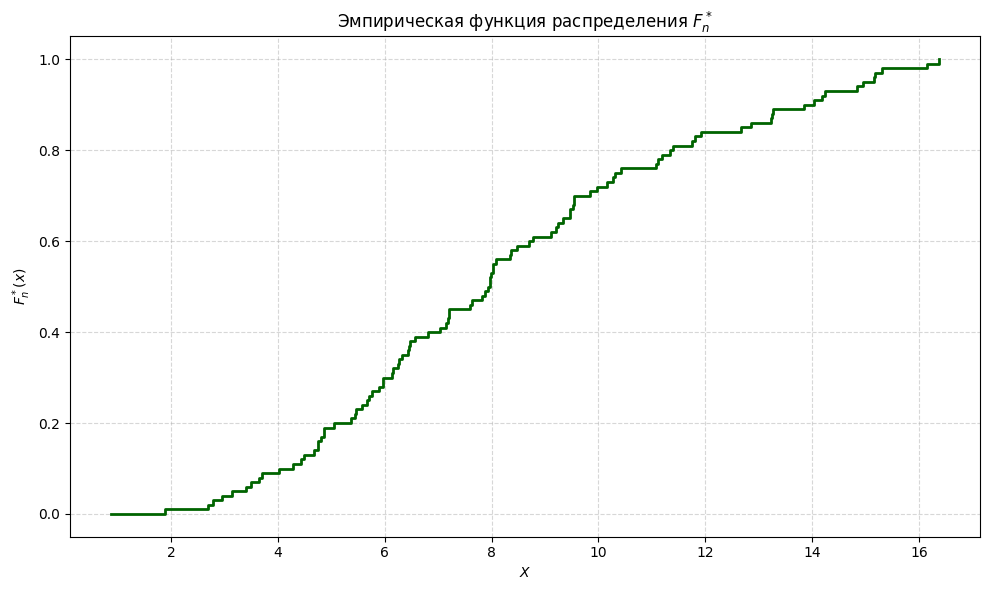
\includegraphics[width=\textwidth]{images/1_ecdf.png}
	\end{figure}

	Код:
	\begin{minted}{python}
		x_sorted = np.sort(X_N)
		y_values = np.arange(1, N + 1) / N
		x_ecdf = np.concatenate(([x_sorted[0] - 1], x_sorted))
		y_ecdf = np.concatenate(([0], y_values))
		plt.figure(figsize=(10, 6))
		plt.step(x_ecdf, y_ecdf, where='post', color='darkgreen', linewidth=2)
		plt.title(r'Эмпирическая функция распределения $F_n^*$')
		plt.xlabel(r'$X$')
		plt.ylabel(r'$F_n^*(x)$')
		plt.ylim(-0.05, 1.05)
		plt.grid(True, linestyle='--', alpha=0.5)
		plt.tight_layout()
	\end{minted}

	\subsection{Выборочные среднее и дисперсия}

	Выборочное среднее вычисляется по формуле:
	\[\displaystyle
	\overline{X}_{18} = \sum_{i = 1}^{N} \frac{x_i}{N} = 8.3139
	\]

	Выборочная дисперсия вычисляется по формуле:
	\[\displaystyle
	\sigma^2_{X_{18}} = \sum_{i = 1}^{N} \frac{(x_i - \overline{X}_{18})^2}{N} = 12.288003789999998
	\]

	Код:
	\begin{minted}{python}
		print(f"Среднее: {np.mean(X_N)}")
		print(f"Дисперсия: {np.var(X_N)}")
	\end{minted}

	\newpage

	\section{задание}
	\subsection{Оценка параметров}

	Оценим параметры равномерного распределения методом максимального правдоподобия: \\
    $\displaystyle
    X \sim U(a, b) \\
    X_1, \ldots, X_n - \text{ выборка из } X \\
    F_X \in \{F(x, a, b) ~|~ a, b \in \mathbb{R}, b \geq a\} \\
    f_X(x) = \frac{I(x \in [a; b])}{(b - a)^n} \\
    L(a, b, X_1, \ldots, X_n) = \prod_{i = 1}^n \frac{I(X_i \in [a; b])}{(b - a)^n} = \frac{1}{(b - a)^n} \prod_{i = 1}^n I(X_i \in [a; b]) \\
    \hat{a}_n = \arg\max_{a \leq b} \frac{1}{(b - a)^n} \prod_{i = 1}^n I(X_i \in [a; b]) = \arg\max_{a \leq X_{\min}} \frac{1}{(b - a)^n} = X_{\min} \\
    \hat{b}_n = \arg\max_{b \geq a} \frac{1}{(b - a)^n} \prod_{i = 1}^n I(X_i \in [a; b]) = \arg\max_{b \geq X_{\max}} \frac{1}{(b - a)^n} = X_{\max} \\
    \text{Оценка параметра } \hat{a}_n = X_{\min} \\
    \text{Оценка параметра } \hat{b}_n = X_{\max} \\
    $

	\subsection{Несмещённость оценки}

	Оценка $\hat{\theta}_n$ является несмещённой, если $E(\hat{\theta}_n) = \theta$

	$\displaystyle
	\text{Математическое ожидание оценки } \hat{a}_n: \\
	P(X_{\min} > x) = P((X_1 > x) \cap \ldots \cap (X_n > x)) = P(X_1 > x) \cdot \ldots \cdot P(X_n > x) \\
	1 - F_{X_{\min}}(x) = 1 - P(X_{\min} \leq x) = (1 - P(X_1 \leq x)) \cdot \ldots \cdot (1 - P(X_n \leq x)) = (1 - F_X(x))^n \\
	F_{X_{\min}}(x) = 1 - (1 - F_X(x))^n \\
	f_{X_{\min}}(x) = \frac{d F_{X_{\min}}}{dx} = n (1 - F_X(x))^{n - 1} f_X(x) = n \left( 1 - \frac{x - a}{b - a} \right)^{n - 1} \frac{1}{b - a} = \frac{n (b - x)^{n - 1}}{(b - a)^n} \\
	E(X_{\min}) = \int_a^b \frac{x n (b - x)^{n - 1}}{(b - a)^n} dx = \frac{na + b}{n + 1} \\
	$

	$\displaystyle
	\text{Математическое ожидание оценки } \hat{b}_n: \\
	F_{X_{\max}}(x) = P(X_{\max} \leq x) = P((X_1 \leq x) \cap \ldots \cap (X_n \leq x)) = P(X_1 \leq x) \cdot \ldots \cdot P(X_n \leq x) = F_X^n(x) \\
	f_{X_{\max}}(x) = \frac{d F_{X_{\max}}}{dx} = n F_X^{n - 1}(x) f_X(x) = n \left( \frac{x - a}{b - a} \right)^{n - 1} \frac{1}{b - a} = \frac{n (x - a)^{n - 1}}{(b - a)^{n}} \\
	E(X_{\max}) = \int_a^b \frac{x n (x - a)^{n - 1}}{(b - a)^{n}} dx = \frac{nb + a}{n + 1} \\
	$
	$
	\left.\begin{array}{c}
		\displaystyle E(\hat{a}_n) = \frac{na + b}{n + 1} \neq a \\
		\displaystyle E(\hat{b}_n) = \frac{nb + a}{n + 1} \neq b
	\end{array}\right\} \Rightarrow
	$
	Оценка смещённая

	\subsection{Состоятельность оценки}

	Оценка $\hat{\theta}_n$ является состоятельной, если $\displaystyle \hat{\theta}_n \xrightarrow{P} \theta \Leftrightarrow \forall \varepsilon > 0 \Rightarrow \lim_{n \rightarrow \infty} P(|\hat{\theta}_n - \theta| < \varepsilon) = 1$

	$\displaystyle
	\text{Предел для оценки } \hat{a}_n: \\
	\lim_{n \rightarrow \infty} P(|\hat{a}_n - a| < \varepsilon) = \lim_{n \rightarrow \infty} P(|X_{\min} - a| < \varepsilon) = \lim_{n \rightarrow \infty} P(X_{\min} - a < \varepsilon) \lim_{n \rightarrow \infty} P(X_{\min} < a + \varepsilon) = \lim_{n \rightarrow \infty} F_{X_{\min}}(a + \varepsilon) = \lim_{n \rightarrow \infty} \left( 1 - \left( \frac{b - a - \varepsilon}{b - a} \right)^n \right) = 1 \\
	$

	$\displaystyle
	\text{Предел для оценки } \hat{b}_n: \\
	\lim_{n \rightarrow \infty} P(|\hat{b}_n - b| < \varepsilon) = \lim_{n \rightarrow \infty} P(|X_{\max} - b| < \varepsilon) = \lim_{n \rightarrow \infty} P(b - X_{\max} < \varepsilon) = \lim_{n \rightarrow \infty} P(X_{\max} > \varepsilon - b) = \lim_{n \rightarrow \infty} (1 - P(X_{\max} \leq b - \varepsilon)) = \lim_{n \rightarrow \infty} (1 - F_{X_{\max}}(b - \varepsilon)) = \lim_{n \rightarrow \infty} \left( 1 - \left( \frac{b - \varepsilon - a}{b - a} \right)^n \right) = 1 \\
	$
	$
	\left.\begin{array}{c}
		\displaystyle \hat{a}_n \xrightarrow{P} a \\
		\displaystyle \hat{b}_n \xrightarrow{P} b
	\end{array}\right\} \Rightarrow
	$
	Оценка состоятельная

	\newpage

	\section{задание}

	\subsection{Входные данные}

	\begin{equation} \label{X_18_3}
		\begin{array}{ccccccccc}
			X: \\
			-3.39 & -1.91 & -19.90 & 14.53 & 10.55 & -5.79 & 14.49 & -3.35 & 1.05 \\
			-1.35 & 18.30 & -7.19 & 12.93 & -9.92 & -5.56 & 15.47 & -6.55 & -8.78 \\
			0.71 & 10.74 & 8.13 & 1.93 & 1.28 & -18.17 & 2.89 & 9.94 & -7.21 \\
			13.70 & -8.66 & 0.11 & 5.89 & 21.52 & 15.33 & 0.23 & -1.02 & -2.98
		\end{array}
	\end{equation}

	\subsection{Вычисление необходимых значений}

	Имеется выборка $X_1, \ldots, X_{36} \text{ из } X \sim N(\mu, \sigma^2)$ 

	Выборочное среднее выборки:
	\[\displaystyle
	\overline{X}_B = 1.888611111111111
	\]

	Исправленное среднеквадратичное отклонение:
	\[\displaystyle
	S = 10.12392474792199
	\]

	Параметр $t$:
	\[\displaystyle
	t = 1.8030237267550329
	\]

	Параметр $q$:
	\[\displaystyle
	q = 0.21050844541225444
	\]

	Код:
	\begin{minted}{python}
		N = len(X_N)
		k = N - 1
		beta = 0.92
		alpha = 1 - beta

		X_mean = np.mean(X_N)
		X_var = np.var(X_N)

		print(f"Среднее: {X_mean}")
		print(f"Дисперсия: {X_var}")
		print(f"Среднеквадратичное отклонение: {np.sqrt(X_var)}")
		print(f"Исправленная дисперсия: {X_var * N / (N - 1)}")
		print(f"Исправленное среднеквадратичное отклонение: {np.sqrt(
		X_var * N / (N - 1))}")

		print(f"t: {scs.t.ppf(1 - alpha / 2, k)}")
		print(f"q: {max(1 - scs.chi.ppf((1 - beta) / 2, k) / 
		(k ** 0.5), scs.chi.ppf((1 + beta) / 2, k) / (k ** 0.5) - 1)}")
	\end{minted}

	\subsection{Точные доверительные интервалы параметров}

	Доверительный интервал параметра $\mu$: \\
	$\displaystyle
	\overline{X}_{B} - t \cdot \frac{S}{\sqrt{N}} < \mu < \overline{X}_{B} + t\frac{S}{\sqrt{N}} \\
	1.89 - 1.8 \cdot \frac{10.12}{6} < \mu < 1.89 + 1.8 \cdot \frac{10.12}{6} \\
	-1.15 < \mu < 4.93
	$

	Доверительный интервал параметра $\sigma$: \\
	$\displaystyle
	S(1 - q) < \sigma < S(1 + q) \\
	10.12 \cdot (1 - 0.21) < \sigma < 10.12 \cdot (1 + 0.21) \\
	7.99 < \sigma < 12.25
	$

	\newpage

	\section{задание}

	Дано: \\
	$\displaystyle
	n = 100 \\
	\overline{D_0} = \frac{1}{n} \sum_{i = 1}^n (x_i - a)^2 \\
	$

	$\displaystyle
	\text{Имеем } n \text{ случайных величин: } x_1, \ldots, x_{n} \sim N(a, \sigma^2) \\
	\frac{x_i - a}{\sigma} \sim N(0, 1), ~~ i = \overline{1, n} \\
	\sum_{i = 1}^{n} \left( \frac{x_i - a}{\sigma} \right)^2 = \frac{\overline{D_0} n}{\sigma^2} = X(n) \sim \chi^2(n) \\
	P\left( \left| \frac{\overline{D_0} - \sigma^2}{\sigma^2} \right| \leq 0.05 \right) = P\left( -0.05 \leq \frac{\overline{D_0} - \sigma^2}{\sigma^2} \leq 0.05 \right) =\\ P\left( -0.05 \leq \frac{\overline{D_0}}{\sigma^2} - 1 \leq 0.05 \right) = P\left( 0.95 \leq \frac{\overline{D_0}}{\sigma^2} \leq 1.05 \right) =\\ P\left( 0.95n \leq \frac{\overline{D_0} n}{\sigma^2} \leq 1.05n \right) = P(95 \leq X(100) \leq 105) = F_{X(100)} (105) - F_{X(100)} (95) \\\approx 0.276
	$

	Код:
	\begin{minted}{python}
		p = scs.chi2.cdf(105, df=100) - scs.chi2.cdf(95, df=100)
		print(f"Вероятность: {p}")
	\end{minted}

	\newpage

	\section{задание}

	\subsection{Входные данные}

	Дано: \\
	$\displaystyle
	\alpha = 0.05 \\
	f(x) = \frac{2a}{(1 + ax)^3}, x \in [0; \infty), a > 0 \\
	$
	\begin{table}[h]
		\begin{tabular}{|c|c|c|c|c|c|c|}
			\hline
			$\Omega_k$ & (0; 1) & (1; 2) & (2; 4) & (4; 6) & (6; 10) & (10; 16) \\ \hline
			$n_k$      & 16     & 16     & 9      & 8      & 6       & 5        \\ \hline
		\end{tabular}
	\end{table}

	\subsection{Проверка гипотезы}

	Необходимо проверить о распределении $X$ по закону с плотностью $f(x)$: \\
	$\displaystyle
	x_k = \frac{a_k + b_k}{2} \\
	x_1 = 0.5; ~~ x_2 = 1.5; ~~ x_3 = 3; ~~ x_4 = 5; ~~ x_5 = 8; ~~ x_6 = 13 \\
	\overline{x}_B = \frac{1}{n} \sum_{i = 1}^6 n_k x_k = \frac{1}{60} (16 \cdot 0.5 + 16 \cdot 1.5 + 9 \cdot 3 + 8 \cdot 5 + 6 \cdot 8 + 5 \cdot 13) = \frac{53}{15} \\
	\text{Сделаем оценку среднего методом моментов:} \\
	E(X) = \overline{x}_B \\
	E(X) = \int_0^{\infty} \frac{2ax}{(1 + ax)^3} dx = 2 \left( \int_0^{\infty} \frac{1}{(1 + ax)^2} dx - \int_0^{\infty} \frac{1}{(1 + ax)^3} dx \right) =\\ 2 \left( \frac{1}{2a (1 + ax)^2} - \frac{1}{a(1 + ax)} \right) \Big|_0^{\infty} = 2 \cdot \frac{1}{2a} = \frac{1}{a} \\
	\frac{1}{a} = \overline{x}_B \\
	a = \frac{1}{\overline{x}_B} = \frac{15}{53} \\
	F(x) = \int_0^x \frac{2a}{(1 + at)^3} dt = -\frac{1}{(1 + at)^2} \Big|_0^x = 1 - \frac{1}{(1 + ax)^2} \\
	p_k = P(x \in \Omega_k) = F(b_k) - F(a_k) = \frac{1}{(1 + a a_k)^2} - \frac{1}{(1 + a b_k)^2} \\
	\text{Для } p_6 \text{ будем брать интервал } (10; \infty) \\
	p_1 \approx 0.3926; ~~ p_2 \approx 0.2; ~~ p_3 \approx 0.1878; ~~ p_4 \approx 0.0826; ~~ p_5 \approx 0.0692; ~~ p_6 \approx 0.0682 \\
	\chi^2_{\text{расч}} = \sum_{i = 1}^6 \frac{(n_i - n p_i)^2}{n p_i} \approx 7.1093 \\
	\chi^2_{\text{табл}}(\alpha = 0.05, k = 4) \approx 9.4877 \\
	\chi^2_{\text{расч}} < \chi^2_{\text{табл}} \Rightarrow \text{гипотеза не отвергается} \\
	p \approx 0.1302
	$

	Код:
	\begin{minted}{python}
		n_k = np.array([16, 16, 9, 8, 6, 5])
		n_k_ = np.array([23.56, 12, 11.268, 4.956, 4.152, 4.092])
		chi2_comp = sum((n_k - n_k_) ** 2 / n_k_)

		print(f"Xи-квадрат расчётная: {chi2_comp}")
		print(f"Xи-квадрат табличная: {scs.chi2.ppf(0.95, 4)}")
		print(f"p-значение: {1 - scs.chi2.cdf(chi2_comp, 4)}")
	\end{minted}

	\newpage

	\section{задание}

	Имеются 2 независимые выборки: \\
	$\displaystyle
	X \sim N(\mu_X, \sigma^2_X); ~~ Y \sim N(\mu_Y, \sigma^2_Y) \\
	n_X = 50; ~~ n_Y = 60 \\
	\overline{X} = 13.2; ~~ \overline{Y} = 14 \\
	D_X = 1.4; ~~ D_Y = 1.2 \\
	H_0: \mu_X = \mu_Y \\
	H_1: \mu_X < \mu_y \\
	t_{\text{расч}} = \frac{|\overline{X} - \overline{Y}|}{\sqrt{(n_X - 1) D_X + (n_Y - 1) D_Y}} \sqrt{\frac{n_X n_Y (n_X + n_Y - 2)}{n_X + n_Y}} =\\ \frac{|13.2 - 14|}{\sqrt{(50 - 1) \cdot 1.4 + (60 - 1) \cdot 1.2}} \sqrt{\frac{50 \cdot 60 (50 + 60 - 2)}{50 + 60}} \approx 3.6774 \\
	t_{\text{табл}}(\alpha = 0.05, k = 50 + 60 - 2) \approx 1.659 \\
	t_{\text{расч}} > t_{\text{табл}} \Rightarrow H_0 \text{ отвергаем}
	$

	\newpage

	\section{задание}

	\subsection{Входные данные}

	\begin{table}[h]
		\begin{tabular}{|c|c|c|c|c|c|c|c|c|c|c|}
			\hline
			$X$ & 9.50 & 7.77 & 17.02 & 4.03 & 7.35 & 11.86 & 16.34 & 6.04 & 7.11 & 7.87 \\ \hline
			$Y$ & -2.66 & 15.55 & -2.86 & 1.73 & 8.73 & -2.21 & 4.02 & -25.54 & -15.73 & -6.25 \\ \hline
		\end{tabular}
		\vspace{0.5cm}
		\vspace{0cm}
		\vspace{0.5cm}
		\begin{tabular}{|c|c|c|c|c|c|c|c|c|c|c|}
			\hline
			$X$ & 6.21 & 13.73 & 3.72 & 11.83 & 6.68 & 9.35 & 8.05 & 11.40 & 5.37 & 14.91 \\ \hline
			$Y$ & -8.44 & 3.74 & 14.81 & -24.90 & 5.41 & -8.47 & 3.61 & -10.95 & -16.91 & -9.06 \\ \hline
		\end{tabular}
		\vspace{0cm}
		\vspace{0cm}
		\vspace{0.5cm}
		\begin{tabular}{|c|c|c|c|c|c|c|c|c|c|c|}
			\hline
			$X$ & 12.05 & 11.95 & 11.29 & 9.56 & 8.51 & 6.29 & 5.17 & 4.46 & 11.07 & 11.80 \\ \hline
			$Y$ & 3.57 & -2.36 & 4.76 & -19.52 & -4.31 & 17.27 & 3.89 & 17.49 & -30.92 & 1.11 \\ \hline
		\end{tabular}
		\begin{tabular}{|c|c|c|c|c|c|c|c|c|c|c|}
			\hline
			$X$ & 11.04 & 7.77 & 9.98 & 2.98 & 10.87 & 10.58 & 8.16 & 7.64 & 9.93 & 8.19 \\ \hline
			$Y$ & 3.39 & 8.79 & 10.20 & 10.21 & -10.21 & -10.70 & -15.26 & -17.87 & 6.92 & -8.66 \\ \hline
		\end{tabular}
	\end{table}

	\subsection{Поле наблюдаемых значений}

	График:
	\begin{figure}[!ht]
		\centering
		\caption{Поле наблюдаемых значений величин $X$ и $Y$}
		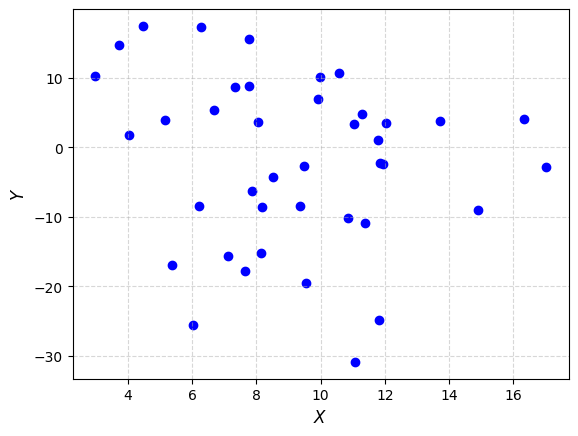
\includegraphics[width=0.8\textwidth]{images/7_plots.png}
	\end{figure}

	Код:
	\begin{minted}{python}
		plt.scatter(x=X, y=Y, color="blue")
		plt.title(r"Поле наблюдаемых значений величин $X$ и $Y$", fontsize=14)
		plt.xlabel(r"$X$", fontsize=12)
		plt.ylabel(r"$Y$", fontsize=12)
		plt.grid(True, linestyle="--", alpha=0.5)

		plt.show()
	\end{minted}

	\subsection{Оценки параметров регрессий}

	\subsubsection{Линейная регрессия}

	Параметры линейной регрессии определяются следующим образом: \\
	$\displaystyle
	y = \alpha_0 + \alpha_1 x \\
	\begin{cases}
		\displaystyle \alpha_0 n + \alpha_1 \sum_{i = 1}^n x_i = \sum_{i = 1}^n y_i & \displaystyle \Big| \times \frac{1}{n} \\
		\displaystyle \alpha_0 \sum_{i = 1}^n x_i + \alpha_1 \sum_{i = 1}^n x_i^2 = \sum_{i = 1}^n y_i x_i
	\end{cases} \Leftrightarrow\\ \begin{cases}
		\displaystyle \alpha_0 = \overline{Y} - \alpha_1 \overline{X} \\
		\displaystyle \overline{Y} \sum_{i = 1}^n x_i - \alpha_1 \overline{X} \sum_{i = 1}^n x_i + \alpha_1 \sum_{i = 1}^n x_i^2 = \sum_{i = 1}^n y_i x_i
	\end{cases} \Leftrightarrow\\ \begin{cases}
		\displaystyle \alpha_0 = \overline{Y} - \alpha_1 \overline{X} \\
		\displaystyle \alpha_1 \left( \sum_{i = 1}^n x_i^2 - \overline{X} \sum_{i = 1}^n x_i \right) = \sum_{i = 1}^n y_i x_i - \overline{Y} \sum_{i = 1}^n x_i & \displaystyle \Big| \times \frac{1}{n}
	\end{cases} \Leftrightarrow\\ \begin{cases}
		\displaystyle \alpha_0 = \overline{Y} - \alpha_1 \overline{X} \\
		\displaystyle \alpha_1 \left( \overline{X^2} - \overline{X}^2 \right) = \overline{YX} - \overline{Y}\, \overline{X}
	\end{cases} \Leftrightarrow \begin{cases}
		\displaystyle \alpha_0 = \overline{Y} - \alpha_1 \overline{X} \\
		\displaystyle \alpha_1 = \frac{\overline{YX} - \overline{Y}\, \overline{X}}{\sigma_X^2}
	\end{cases} \Leftrightarrow\\ \begin{cases}
		\alpha_0 = 3.537878636317131 \\
		\alpha_1 = -0.6258521343422414
	\end{cases}
	$

	\subsubsection{Квадратичная регрессия}

	Параметры квадратичной регрессии определяются следующим образом: \\
	$\displaystyle
	y = \beta_0 + \beta_1 x + \beta_2 x^2 \\
	\begin{cases}
		\displaystyle \beta_0 n + \beta_1 \sum_{i = 1}^n x_i + \beta_2 \sum_{i = 1}^n x_i^2 = \sum_{i = 1}^n y_i & \displaystyle \Big| \times \frac{1}{n} \\
		\displaystyle \beta_0 \sum_{i = 1}^n x_i + \beta_1 \sum_{i = 1}^n x_i^2 + \beta_2 \sum_{i = 1}^n x_i^3 = \sum_{i = 1}^n y_i x_i \\
		\displaystyle \beta_0 \sum_{i = 1}^n x_i^2 + \beta_1 \sum_{i = 1}^n x_i^3 + \beta_2 \sum_{i = 1}^n x_i^4 = \sum_{i = 1}^n y_i x_i^2
	\end{cases} \Leftrightarrow\\ \begin{cases}
		\displaystyle \beta_0 = \overline{Y} - \beta_1 \overline{X} - \beta_2 \overline{X^2} \\
		\displaystyle \overline{Y} \sum_{i = 1}^n x_i - \beta_1 \overline{X} \sum_{i = 1}^n x_i + \beta_1 \sum_{i + 1}^n x_i^2 - \beta_2 \overline{X^2} \sum_{i = 1}^n x_i + \beta_2 \sum_{i = 1}^n x_i^3 = \sum_{i = 1}^n y_i x_i & \displaystyle \Big| \times \frac{1}{n} \\
		\displaystyle \overline{Y} \sum_{i = 1}^n x_i^2 - \beta_1 \overline{X} \sum_{i = 1}^n x_i^2 + \beta_1 \sum_{i = 1}^n x_i^3 - \beta_2 \overline{X^2} \sum_{i = 1}^n x_i^2 + \beta_2 \sum_{i = 1}^n x_i^4 = \sum_{i = 1}^n y_i x_i^2
	\end{cases} \Leftrightarrow\\ \begin{cases}
		\displaystyle \beta_0 = \overline{Y} - \beta_1 \overline{X} - \beta_2 \overline{X^2} \\
		\displaystyle \overline{Y}\, \overline{X} - \beta_1 \overline{X}^2 + \beta_1 \overline{X^2} - \beta_2 \overline{X^2}\, \overline{X} + \beta_2 \overline{X^3} = \overline{YX} \\
		\displaystyle \overline{Y} \sum_{i = 1}^n x_i^2 - \beta_1 \overline{X} \sum_{i = 1}^n x_i^2 + \beta_1 \sum_{i = 1}^n x_i^3 - \beta_2 \overline{X^2} \sum_{i = 1}^n x_i^2 + \beta_2 \sum_{i = 1}^n x_i^4 = \sum_{i = 1}^n y_i x_i^2
	\end{cases} \Leftrightarrow\\ \begin{cases}
		\displaystyle \beta_0 = \overline{Y} - \beta_1 \overline{X} - \beta_2 \overline{X^2} \\
		\displaystyle \beta_1 \left( \overline{X^2} - \overline{X}^2 \right) = \overline{YX} - \overline{Y}\, \overline{X} + \beta_2 \overline{X^2}\, \overline{X} - \beta_2 \overline{X^3} \\
		\displaystyle \overline{Y} \sum_{i = 1}^n x_i^2 - \beta_1 \overline{X} \sum_{i = 1}^n x_i^2 + \beta_1 \sum_{i = 1}^n x_i^3 - \beta_2 \overline{X^2} \sum_{i = 1}^n x_i^2 + \beta_2 \sum_{i = 1}^n x_i^4 = \sum_{i = 1}^n y_i x_i^2
	\end{cases} \Leftrightarrow\\ \begin{cases}
		\displaystyle \beta_0 = \overline{Y} - \beta_1 \overline{X} - \beta_2 \overline{X^2} \\
		\displaystyle \beta_1 = \frac{\overline{YX} - \overline{Y}\, \overline{X} + \beta_2 \overline{X^2}\, \overline{X} - \beta_2 \overline{X^3}}{\sigma_X^2} \\
		\left.\begin{array}{l}
			\displaystyle \overline{Y} \sum_{i = 1}^n x_i^2 + \frac{\overline{YX}}{\sigma_X^2} \sum_{i = 1}^n x_i^3 - \frac{\overline{Y}\, \overline{X}}{\sigma_X^2} \sum_{i = 1}^n x_i^3 - \frac{\overline{YX}\, \overline{X}}{\sigma_X^2} \sum_{i = 1}^n x_i^2 +\\\displaystyle+ \frac{\overline{Y}\, \overline{X}^2}{\sigma_X^2} \sum_{i = 1}^n x_i^2 - \beta_2 \frac{\overline{X^3}}{\sigma_X^2} \sum_{i = 1}^n x_i^3 + \beta_2 \frac{\overline{X^2}\, \overline{X}}{\sigma_X^2} \sum_{i = 1}^n x_i^3 + \beta_2 \frac{\overline{X^3}\, \overline{X}}{\sigma_X^2} \sum_{i = 1}^n x_i^2 -\\\displaystyle- \beta_2 \frac{\overline{X^2}\, \overline{X}^2}{\sigma_X^2} \sum_{i = 1}^n x_i^2 - \beta_2 \overline{X^2} \sum_{i = 1}^n x_i^2 + \beta_2 \sum_{i = 1}^n x_i^4 = \sum_{i = 1}^n y_i x_i^2
		\end{array}\right| \displaystyle \times \frac{1}{n}
	\end{cases} \Leftrightarrow \begin{cases}
		\displaystyle \beta_0 = \overline{Y} - \beta_1 \overline{X} - \beta_2 \overline{X^2} \\
		\displaystyle \beta_1 = \frac{\overline{YX} - \overline{Y}\, \overline{X} + \beta_2 \overline{X^2}\, \overline{X} - \beta_2 \overline{X^3}}{\sigma_X^2} \\
		\displaystyle \overline{Y}\, \overline{X^2} + \frac{\overline{YX}\, \overline{X^3}}{\sigma_X^2} - \frac{\overline{Y}\, \overline{X}\, \overline{X^3}}{\sigma_X^2} - \frac{\overline{YX}\, \overline{X}\, \overline{X^2}}{\sigma_X^2} + \frac{\overline{Y}\, \overline{X}^2\, \overline{X^2}}{\sigma_X^2} - \beta_2 \frac{\overline{X^3}^2}{\sigma_X^2} +\\\displaystyle+ \beta_2 \frac{\overline{X^2}\, \overline{X}\, \overline{X^3}}{\sigma_X^2} + \beta_2 \frac{\overline{X^3}\, \overline{X}\, \overline{X^2}}{\sigma_X^2} - \beta_2 \frac{\overline{X^2}\, \overline{X}^2\, \overline{X^2}}{\sigma_X^2} - \beta_2 \overline{X^2}^2 + \beta_2 \overline{X^4} = \overline{YX^2}
	\end{cases} \Leftrightarrow\\ \begin{cases}
		\displaystyle \beta_0 = \overline{Y} - \beta_1 \overline{X} - \beta_2 \overline{X^2} \\
		\displaystyle \beta_1 = \frac{\overline{YX} - \overline{Y}\, \overline{X} + \beta_2 \overline{X^2}\, \overline{X} - \beta_2 \overline{X^3}}{\sigma_X^2} \\
		\displaystyle \beta_2 \left( \frac{\overline{X^2}\, \overline{X}\, \overline{X^3}}{\sigma_X^2} - \frac{\overline{X^3}^2}{\sigma_X^2} + \frac{\overline{X^3}\, \overline{X}\, \overline{X^2}}{\sigma_X^2} - \frac{\overline{X^2}\, \overline{X}^2\, \overline{X^2}}{\sigma_X^2} - \overline{X^2}^2 + \overline{X^4} \right) =\\\displaystyle= \overline{YX^2} - \overline{Y}\, \overline{X^2} - \frac{\overline{YX}\, \overline{X^3}}{\sigma_X^2} + \frac{\overline{Y}\, \overline{X}\, \overline{X^3}}{\sigma_X^2} + \frac{\overline{YX}\, \overline{X}\, \overline{X^2}}{\sigma_X^2} - \frac{\overline{Y}\, \overline{X}^2\, \overline{X^2}}{\sigma_X^2}
	\end{cases} \Leftrightarrow\\ \begin{cases}
		\displaystyle \beta_0 = \overline{Y} - \beta_1 \overline{X} - \beta_2 \overline{X^2} \\
		\displaystyle \beta_1 = \frac{\overline{YX} - \overline{Y}\, \overline{X} + \beta_2 \overline{X^2}\, \overline{X} - \beta_2 \overline{X^3}}{\sigma_X^2} \\
		\displaystyle \beta_2 \left( \sigma_{X^2}^2 - \frac{\left( \overline{X^3} - \overline{X^2}\, \overline{X} \right)^2}{\sigma_X^2} \right) =\\\displaystyle= \overline{YX^2} - \overline{Y}\, \overline{X^2} + \frac{-\overline{YX}\, \overline{X^3} + \overline{Y}\, \overline{X}\, \overline{X^3} + \overline{YX}\, \overline{X}\, \overline{X^2} - \overline{Y}\, \overline{X}^2\, \overline{X^2}}{\sigma_X^2}
	\end{cases} \Leftrightarrow\\ \begin{cases}
		\displaystyle \beta_0 = \overline{Y} - \beta_1 \overline{X} - \beta_2 \overline{X^2} \\
		\displaystyle \beta_1 = \frac{\overline{YX} - \overline{Y}\, \overline{X} + \beta_2 \overline{X^2}\, \overline{X} - \beta_2 \overline{X^3}}{\sigma_X^2} \\
		\displaystyle \beta_2 \frac{\sigma_{X^2}^2 \sigma_X^2 - \left( \overline{X^3} - \overline{X^2}\, \overline{X} \right)^2}{\sigma_X^2} = \overline{YX^2} - \overline{Y}\, \overline{X^2} - \frac{\left( \overline{YX} - \overline{Y}\, \overline{X} \right) \left( \overline{X^3} - \overline{X^2}\, \overline{X} \right)}{\sigma_X^2}
	\end{cases} \Leftrightarrow \begin{cases}
		\displaystyle \beta_0 = \overline{Y} - \beta_1 \overline{X} - \beta_2 \overline{X^2} \\
		\displaystyle \beta_1 = \frac{\overline{YX} - \overline{Y}\, \overline{X} + \beta_2 \overline{X^2}\, \overline{X} - \beta_2 \overline{X^3}}{\sigma_X^2} \\
		\displaystyle \beta_2 = \frac{\sigma_X^2 \left( \overline{YX^2} - \overline{Y}\, \overline{X^2} \right) - \left( \overline{YX} - \overline{Y}\, \overline{X} \right) \left( \overline{X^3} - \overline{X^2}\, \overline{X} \right)}{\sigma_{X^2}^2 \sigma_X^2 - \left( \overline{X^3} - \overline{X^2}\, \overline{X} \right)^2}
	\end{cases} \Leftrightarrow\\ \begin{cases}
		\beta_0 = 20.18790228082293 \\
		\beta_1 = -4.533721095855133 \\
		\beta_2 = 0.20241886078821292
	\end{cases}
	$

	\subsubsection{Код}

	\begin{minted}{python}
		X_mean = np.mean(X)
		X2_mean = np.mean(X ** 2)
		X3_mean = np.mean(X ** 3)

		Y_mean = np.mean(Y)
		YX_mean = np.mean(Y * X)
		YX2_mean = np.mean(Y * X ** 2)

		X_var = np.var(X)
		X2_var = np.var(X ** 2)

		alpha_1 = (YX_mean - Y_mean * X_mean) / X_var
		alpha_0 = Y_mean - alpha_1 * X_mean
		y_lin = lambda x: alpha_0 + alpha_1 * x

		beta_2 = (X_var * (YX2_mean - Y_mean * X2_mean) - (YX_mean - Y_mean * X_mean) * (X3_mean - X2_mean * X_mean)) / (X2_var * X_var - (X3_mean - X2_mean * X_mean) ** 2)
		beta_1 = (YX_mean - Y_mean * X_mean + beta_2 * X2_mean * X_mean - beta_2 * X3_mean) / X_var
		beta_0 = Y_mean - beta_1 * X_mean - beta_2 * X2_mean
		y_sqr = lambda x: beta_0 + beta_1 * x + beta_2 * x ** 2

		print(f"Коэффициенты линейной регрессии: alpha_0 = {alpha_0}, 
		alpha_1 = {alpha_1}")
		print(f"Коэффициенты квадратичной регрессии: beta_0 = 
		{beta_0}, beta_1 = {beta_1}, beta_2 = {beta_2}\n")
	\end{minted}

	\subsection{Проверка гипотезы о значимости параметров регрессии}

	\subsubsection{Линейная регрессия}

	Проверка гипотезы о значимости коэффициентов линейной регрессии: \\
	$\displaystyle
	H_0: \alpha_0 = \alpha_1 = 0 \\
	H_1: \alpha_0 \neq 0; ~ \alpha_1 \neq 0 \\
	S_{\text{ост}}^2 = \sum_{i = 1}^n \frac{(y_i - \hat{y}_{x_i})^2}{n - 2} \\
	m_{\alpha_0} = \frac{S_{\text{ост}} \sqrt{\displaystyle \sum_{i = 1}^n x_i^2}}{n \sigma_x}; ~~
	m_{\alpha_1} = \frac{S_{\text{ост}}}{\sigma_x \sqrt{n}} \\
	t_{\alpha_0} = \frac{\alpha_0}{m_{\alpha_0}}; ~~
	t_{\alpha_1} = \frac{\alpha_1}{m_{\alpha_1}} \\
	\left.\begin{array}{l}
		t_{\alpha_0} \approx 0.6 \\
		t_{\alpha_1} \approx -1.1
	\end{array}\right\} < t_{\text{табл}}(\alpha = 0.05, k = n - 2) \approx 1.6 \Rightarrow H_0 \text{ не отвергаем}
	$

	\subsubsection{Квадратичная регрессия}

	Проверка гипотезы о значимости коэффициентов квадратичной регрессии: \\
	$\displaystyle
	H_0: \beta_0 = \beta_1 = \beta_2 = 0 \\
	H_1: \beta_0 \neq 0; ~ \beta_1 \neq 0; ~ \beta_2 \neq 0 \\
	S_{\text{ост}}^2 = \sum_{i = 1}^n \frac{(y_i - \hat{y}_{x_i})^2}{n - 3} \\
	V = \left(\begin{array}{ccc}
		n & \displaystyle \sum_{i = 1}^n x_i & \displaystyle \sum_{i = 1}^n x_i^2 \\
		\displaystyle \sum_{i = 1}^n x_i & \displaystyle \sum_{i = 1}^n x_i^2 & \displaystyle \sum_{i = 1}^n x_i^3 \\
		\displaystyle \sum_{i = 1}^n x_i^2 & \displaystyle \sum_{i = 1}^n x_i^3 & \displaystyle \sum_{i = 1}^n x_i^4 \\
	\end{array}\right) \\
	V^{-1} = \left(\begin{array}{ccc}
		C_{00} & C_{01} & C_{02} \\
		C_{10} & C_{11} & C_{12} \\
		C_{20} & C_{21} & C_{22}
	\end{array}\right) \\
	m_{\beta_0} = S_{\text{ост}} \sqrt{C_{00}}; ~~
	m_{\beta_1} = S_{\text{ост}} \sqrt{C_{11}}; ~~
	m_{\beta_2} = S_{\text{ост}} \sqrt{C_{22}} \\
	t_{\beta_0} = \frac{\beta_0}{m_{\beta_0}}; ~~
	t_{\beta_1} = \frac{\beta_1}{m_{\beta_1}}; ~~
	t_{\beta_2} = \frac{\beta_2}{m_{\beta_2}} \\
	\left.\begin{array}{l}
		t_{\beta_0} \approx 1.6 \\
		t_{\beta_1} \approx -1.7 \\
		t_{\beta_2} \approx 1.5
	\end{array}\right\} < t_{\text{табл}}(\alpha = 0.05, k = n - 3) \approx 1.7 \Rightarrow H_0 \text{ не отвергаем}
	$

	\subsection{Коэффициент детерминации}

	Коэффициент детерминации вычисляется по формуле: \\
	$\displaystyle
	R^2 = 1 - \frac{\displaystyle \sum_{i = 1}^n (y_i - \hat{y}_{x_i})^2}{\displaystyle \sum_{i = 1}^n (y_i - \overline{Y})^2} \\
	$
	Для линейной модели $R^2 \approx 0.03 \Rightarrow$ модель очень плохо описывает данные $X$ и $Y$.
	Для квадратичной модели $R^2 \approx 0.08 \Rightarrow$ модель очень плохо описывает данные $X$ и $Y$ 

	Код:
	\begin{minted}{python}
		S = np.sum((Y - Y_mean) ** 2)
		R2_lin = 1 - np.sum((Y - np.array([y_lin(x) for x in X])) ** 2) / S
		R2_sqr = 1 - np.sum((Y - np.array([y_sqr(x) for x in X])) ** 2) / S

		print(f"R^2 для линейной модели: {R2_lin}")
		print(f"R^2 для квадратичной модели: {R2_sqr}")
	\end{minted}

	\subsection{Графики полученных моделей}

	График:
	\begin{figure}[H]
		\centering
		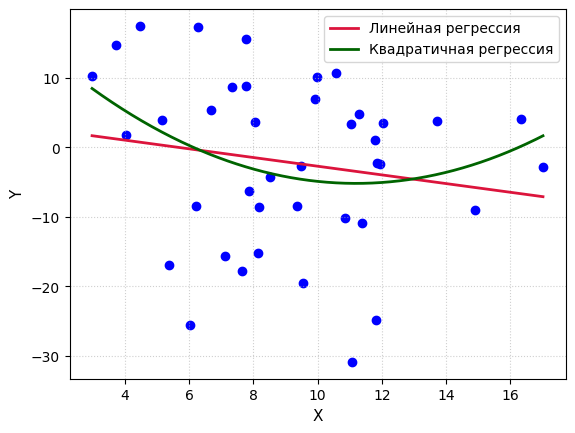
\includegraphics[width=0.8\textwidth]{images/7_regressions.png}
		\caption{Сравнение линейной и квадратичной регрессий на фоне корреляционного поля}
		\label{fig:graph}
	\end{figure}

	Код:
	\begin{minted}{python}
		x_plots = np.linspace(min(X), max(X), 500)

		y_lin_plots = alpha_0 + alpha_1 * x_plots
		y_sqr_plots = beta_0 + beta_1 * x_plots + beta_2 * (x_plots ** 2)

		plt.scatter(x=X, y=Y, color="blue")
		plt.plot(
			x_plots,
			y_lin_plots,
			color="crimson",
			linestyle="-",
			linewidth=2,
			label=f"Линейная регрессия",
		)
		plt.plot(
			x_plots,
			y_sqr_plots,
			color="darkgreen",
			linestyle="-",
			linewidth=2,
			label=f"Квадратичная регрессия",
		)

		plt.xlabel("X", fontsize=11)
		plt.ylabel("Y", fontsize=11)
		plt.grid(True, linestyle=":", alpha=0.6)
		plt.legend(fontsize=10)

		plt.show()
	\end{minted}

\end{document}